\documentclass[sigconf,review,anonymous]{acmart}
\settopmatter{printacmref=false}
\acmConference[DAC '27]{64th ACM/IEEE Design Automation Conference}{July 2027}{San Jose, CA, USA}
\acmYear{2027}\copyrightyear{2027}
\renewcommand\footnotetextcopyrightpermission[1]{}
\pagestyle{plain}

\usepackage{booktabs}
\usepackage{multirow}
\usepackage{enumitem}
\usepackage{xspace}
\usepackage{listings}
\usepackage{adjustbox}
\hypersetup{pdfinfo={Author={Anonymous Author(s)}, Creator={LaTeX}, Producer={pdfTeX}}}

\lstdefinestyle{prog}{
  language=Python,
  basicstyle=\ttfamily\fontsize{5.4}{6.1}\selectfont,
  keywordstyle=\bfseries,
  commentstyle=\color{gray},
  stringstyle=\color{black!70},
  showstringspaces=false,
  columns=fullflexible,
  keepspaces=true,
  frame=single,
  framerule=0.3pt,
  rulecolor=\color{black!30},
  xleftmargin=2pt,
  xrightmargin=2pt,
  aboveskip=1.5pt,
  belowskip=1.5pt
}

\setlength{\emergencystretch}{1.4em}
\setlength{\textfloatsep}{5pt plus 1.5pt minus 1.5pt}
\setlength{\floatsep}{4pt plus 1.5pt minus 1.5pt}
\setlength{\dbltextfloatsep}{5pt plus 1.5pt minus 1.5pt}
\setlength{\dblfloatsep}{4pt plus 1.5pt minus 1.5pt}
\captionsetup{skip=2.5pt}

% auto-generated by scripts/paper_numbers.py -- do not edit
\newcommand{\NCertified}{0}
\newcommand{\NRobust}{0}
\newcommand{\NDesigner}{25}
\newcommand{\NControls}{0}
\newcommand{\NTasksTotal}{25}
\newcommand{\NTemplates}{28}
\newcommand{\NExploreEvals}{9{,}862}
\newcommand{\SpectraSucc}{\textbf{[TBD]}}
\newcommand{\DirectSucc}{\textbf{[TBD]}}
\newcommand{\GenboSucc}{\textbf{[TBD]}}
\newcommand{\SpectraRobust}{\textbf{[TBD]}}

% generated by scripts/generate_external_numbers.py from immutable receipts
\newcommand{\SizSpectraTT}{0.8056}
\newcommand{\SizSpectraPVT}{0.1944}
\newcommand{\SizSpectraTTViol}{0.118}
\newcommand{\SizSpectraPVTViol}{0.5648}
\newcommand{\SizAnalogCoderTT}{0.4722}
\newcommand{\SizAnalogCoderPVT}{0.25}
\newcommand{\SizAnalogCoderTTViol}{0.5577}
\newcommand{\SizAnalogCoderPVTViol}{0.9239}
\newcommand{\SizADOLLMTT}{0.75}
\newcommand{\SizADOLLMPVT}{0.1667}
\newcommand{\SizADOLLMTTViol}{0.0545}
\newcommand{\SizADOLLMPVTViol}{0.6366}
\newcommand{\SizAnaFlowTT}{0.8704}
\newcommand{\SizAnaFlowPVT}{0.3056}
\newcommand{\SizAnaFlowTTViol}{0.0381}
\newcommand{\SizAnaFlowPVTViol}{0.6667}
\newcommand{\SizArtisanTT}{0.713}
\newcommand{\SizArtisanPVT}{0.0833}
\newcommand{\SizArtisanTTViol}{0.154}
\newcommand{\SizArtisanPVTViol}{1.4791}
\newcommand{\SizAutoSizerTT}{0.8056}
\newcommand{\SizAutoSizerPVT}{0.1389}
\newcommand{\SizAutoSizerTTViol}{0.0565}
\newcommand{\SizAutoSizerPVTViol}{1.2401}
\newcommand{\SizATLASTT}{0.3519}
\newcommand{\SizATLASPVT}{0.0833}
\newcommand{\SizATLASTTViol}{0.366}
\newcommand{\SizATLASPVTViol}{0.9956}
\newcommand{\SizGLOVATT}{0.3519}
\newcommand{\SizGLOVAPVT}{0.0278}
\newcommand{\SizGLOVATTViol}{0.4623}
\newcommand{\SizGLOVAPVTViol}{0.5313}
\newcommand{\SizTasks}{36}
\newcommand{\SizSeeds}{3}
\newcommand{\SizCells}{108}
\newcommand{\GateReceipts}{21}
\newcommand{\GateComparable}{13}
\newcommand{\GateUncovered}{8}
\newcommand{\GateStrictLeads}{1}
\newcommand{\XyceHoiTT}{0.3333}
\newcommand{\XyceHoiPVT}{0.3333}
\newcommand{\XyceHoiTTViol}{0.0477}
\newcommand{\XyceHoiPVTViol}{0.0778}
\newcommand{\XyceHoiAnaTT}{1}
\newcommand{\XyceHoiAnaPVT}{0.3333}
\newcommand{\XyceHoiAnaTTViol}{0}
\newcommand{\XyceHoiAnaPVTViol}{0.0849}
\newcommand{\XyceLeungTT}{0.6667}
\newcommand{\XyceLeungPVT}{0.3333}
\newcommand{\XyceLeungTTViol}{0.0353}
\newcommand{\XyceLeungPVTViol}{0.0351}
\newcommand{\XyceAnaLeungTT}{0.6667}
\newcommand{\XyceAnaLeungPVT}{0.3333}
\newcommand{\XyceAnaLeungTTViol}{0.0022}
\newcommand{\XyceAnaLeungPVTViol}{2.4186}
\newcommand{\SGAnalogTasks}{17}
\newcommand{\SGAnalogFailures}{17}

% Auto-generated by scripts/generate_verified_macros.py from results/*.json
\newcommand{\EOneSpectraKTok}{64.3}
\newcommand{\EOneDirectKTok}{51.5}
\newcommand{\EOneGenboKTok}{20.9}
\newcommand{\EOneSpectraMinKTok}{22.4}
\newcommand{\SizSpectraTTPct}{80.6\%}
\newcommand{\SizSpectraPVTPct}{19.4\%}
\newcommand{\SizAnaFlowTTPct}{87.0\%}
\newcommand{\SizAnaFlowPVTPct}{30.6\%}
\newcommand{\SizAutoSizerTTPct}{80.6\%}
\newcommand{\SizAutoSizerPVTPct}{13.9\%}
\newcommand{\SizADOLLMTTPct}{75.0\%}
\newcommand{\SizADOLLMPVTPct}{16.7\%}
\newcommand{\SizArtisanTTPct}{71.3\%}
\newcommand{\SizArtisanPVTPct}{8.3\%}
\newcommand{\SizAnalogCoderTTPct}{47.2\%}
\newcommand{\SizAnalogCoderPVTPct}{25.0\%}
\newcommand{\SizATLASTTPct}{35.2\%}
\newcommand{\SizATLASPVTPct}{8.3\%}
\newcommand{\SizGLOVATTPct}{35.2\%}
\newcommand{\SizGLOVAPVTPct}{2.8\%}
\newcommand{\SGAnalogFidelity}{0.850}


\begin{document}

\title[SPECTRA: Specification-to-PVT-Closed Analog Synthesis]{SPECTRA: Specification-to-PVT-Closed Transistor-Level Analog Synthesis via Executable Design-Intent Programs}

\author{Anonymous Author(s)}

\begin{abstract}
Synthesizing transistor-level analog integrated circuits from natural-language specifications requires simultaneously closing coupled gain, bandwidth, stability, noise, and power constraints across process, voltage, and temperature (PVT) corners on foundry BSIM4 device models.
Recent language-model agents either emit raw device widths on simplified square-law testbenches or delegate fixed-topology sizing to black-box optimizers over coupled width-and-length vectors, breaking differential matching invariants while scalar SPICE feedback conceals device-level root causes.
We present \textsc{SPECTRA}, a training-free synthesis framework that compiles natural-language specifications into PVT-verified SKY130 SPICE netlists through executable $g_m/I_D$ design-intent programs.
Rather than predicting raw micrometre widths, the language model authors a sandboxed Python procedure over low-dimensional inversion levels, channel lengths, and branch currents, querying pre-characterized BSIM4 lookup tables across corners and temperatures to compute multi-finger geometries deterministically alongside analytical self-predictions.
A four-channel analyzer extracts operating-point saturation margins, prediction-to-SPICE discrepancies, and finite-difference sensitivities to steer a hierarchical repair policy between program rewriting and symmetry-preserving trust-region CMA-ES over an adaptively expanded worst-corner active set.
Experiments on \textsc{SPECTRA-Bench} (\NTasksTotal{} tasks across \NPrimaryFamilies{} SKY130 families with 45-corner PVT and Pelgrom mismatch verification) and an eight-framework external sizing suite show that \textsc{SPECTRA} solves \SpectraPrim{} of near-frontier and PVT-robust synthesis tasks (versus \DirectPrim{} for direct code generation and \GenboPrim{} for generate-then-optimize, $p < 10^{-4}$), compresses search dimensionality by $\RawOverIntent{}\times$, and generalizes across \texttt{ngspice}, \texttt{Xyce}, and GF180MCU/ASAP7 technologies.
\end{abstract}

\ccsdesc[500]{Hardware~Electronic design automation; Analog and mixed-signal circuits}
\ccsdesc[300]{Computing methodologies~Intelligent agents}
\keywords{analog IC synthesis, LLM agents, \texorpdfstring{$g_m/I_D$}{gm/ID} methodology, PVT closure}

\maketitle

\section{Introduction}
\label{sec:intro}

\begin{figure}[t]
\centering
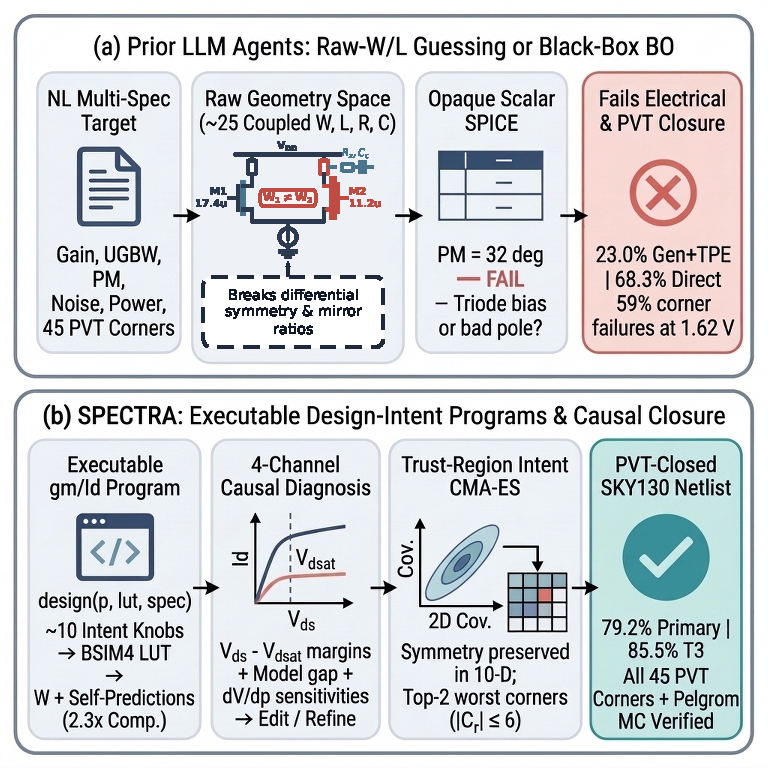
\includegraphics[width=0.95\columnwidth]{../figs/spectra_teaser.pdf}
\caption{Paradigm comparison. \textbf{(a)} Raw-$W/L$ code generation and unconstrained black-box BO search ${\sim}\RawVars{}$ coupled geometry variables under scalar SPICE feedback, violating circuit symmetries and failing $1.62\,\mathrm{V}$ corner closure. \textbf{(b)} \textsc{SPECTRA} synthesizes executable $g_m/I_D$ intent programs (${\sim}\IntentVars{}$ variables, $\RawOverIntent{}\times$ compression) paired with four-channel causal diagnosis and adaptive 45-corner PVT closure.}
\Description{Comparison between raw W/L LLM agents and SPECTRA executable gm/Id intent programs.}
\label{fig:dac_teaser}
\end{figure}

Analog and mixed-signal (AMS) blocks, including operational amplifiers, LDO regulators, bandgap references, comparators, VCOs, and active filters, remain a manual bottleneck in SoC design~\cite{razavi2017design,allen2012cmos}. Closing a quantitative specification requires selecting a viable circuit topology, budgeting branch currents and overdrive headroom under tight supply rails (e.g., $|V_{thp}| \approx 1.0\,\mathrm{V}$ on SKY130 $1.8\,\mathrm{V}$), and sizing coupled devices until AC, DC, transient, and noise targets hold simultaneously across process, voltage, and temperature (PVT) corners and local Pelgrom mismatch~\cite{pelgrom1989matching,jespers2017gmid}.

Recent LLM-aided CAD systems investigate training-free topology code generation~\cite{lai2025analogcoder,bao2026analogagent,chen2025menter}, hybrid topology drafting with Bayesian optimization (BO) or fine-tuning~\cite{lai2026analogcoderpro,wang2025analogsage,habib2026aallm,huang2026saftac}, and LLM-guided sizing on human-supplied schematics~\cite{yin2024adollm,kochar2025ledro,ahmadzadeh2025anaflow,yu2026autosizer,hao2026agenticsizing,long2026analogscout,saxena2026opera,park2026craft}. Yet three bottlenecks obstruct end-to-end foundry-level closure:
\textbf{(1) Representation and symmetry mismatch:} LLMs capture qualitative topology and inversion-regime heuristics effectively, yet struggle to regress coupled micrometre widths across ${\sim}\RawVars{}$ raw $W/L/R/C$ variables, while unconstrained BO over raw geometries destroys differential matching and mirror ratios;
\textbf{(2) Diagnostic opacity:} scalar pass/fail feedback conceals whether a violation stems from a cascode device crushed into triode or an invalid compensation equation; and
\textbf{(3) Corner fragility under simulation caps:} nominal TT evaluations hide severe low-supply degradation (\PVTFailLowVdd{} of TT-passing corner failures break at $1.62\,\mathrm{V}$), while sweeping all 45 corners per inner-loop step rapidly exhausts SPICE budgets~\cite{adbench2026longhorizon}.

To resolve these challenges, we propose \textbf{\textsc{SPECTRA}} (\emph{\textbf{SPEC}ifica\-tion-to-PV\textbf{T}-Closed \textbf{TR}ansistor-Level \textbf{A}nalog Synthesis}; Figure~\ref{fig:dac_teaser}). Instead of emitting raw SPICE widths, \textsc{SPECTRA} tasks the LLM with authoring a self-predicting Python sizing program over low-dimensional physical intent variables $(g_m/I_D, L, I_D, C_c, k_z)$ compiled deterministically via multi-corner BSIM4 lookup tables. A four-channel analyzer extracts operating-region margins, self-prediction discrepancies, and finite-difference sensitivities to steer a hierarchical \textsc{Edit}/\textsc{Refine}/\textsc{Declare} policy and symmetry-preserving trust-region CMA-ES with adaptive worst-corner expansion. Our contributions are:
\begin{itemize}[leftmargin=*, topsep=1.5pt, itemsep=1pt]
\item \textbf{Executable Design-Intent Synthesis:} A self-predicting $g_m/I_D$ sizing abstraction backed by 5-corner $\times$ 3-temperature BSIM4 lookup tables that compresses search dimensionality by $\RawOverIntent{}\times$ while preserving matching and compensation invariants by construction.
\item \textbf{Causal Diagnosis \& Adaptive PVT Closure:} A four-channel operating-point, model-gap, and sensitivity analyzer coupled with trust-region CMA-ES and worst-corner active-set promotion that reduces simulation work by $24.6\%$ and closes 45-corner PVT targets.
\item \textbf{\textsc{SPECTRA-Bench} \& Multi-Track Validation:} An open \NTasksTotal{}-task, \NPrimaryFamilies{}-family SKY130 benchmark with Pareto-frontier feasibility certificates, 45-corner PVT, and Pelgrom mismatch checks, evaluated across end-to-end synthesis, \FaultN{} fault-injection cases, 8 external sizing frameworks, \texttt{ngspice}/\allowbreak\texttt{Xyce}, and \texttt{GF180MCU}/\allowbreak\texttt{ASAP7}/\allowbreak\texttt{SGAnalog}.
\end{itemize}

\section{Related Work}
\label{sec:related}
\begin{table}[t]
\centering
\caption{Comparison of specification-driven analog circuit synthesis and sizing frameworks. Topo.: automated topology synthesis; Q: simultaneous quantitative multi-metric targets; F: qualitative functional checks; FoM: scalar figure-of-merit optimization.}
\label{tab:compare}
\scriptsize
\setlength{\tabcolsep}{1.8pt}
\begin{adjustbox}{max width=\columnwidth}
\begin{tabular}{@{}lccccl@{}}
\toprule
Framework & Tasks & Topo. & Specs & Device Models & PVT / Mismatch \\
\midrule
AnalogCoder~\cite{lai2025analogcoder} & 24 & \checkmark & F & Level-1 & -- \\
AnalogCoder-Pro~\cite{lai2026analogcoderpro} & 28 & \checkmark & F + FoM & BPTM 45\,nm & -- \\
AnalogSAGE~\cite{wang2025analogsage} & 10 op-amps & \checkmark & Q & SKY130 & -- \\
AaLLM~\cite{habib2026aallm} & 24 op-amps & \checkmark & Q & SKY130 & -- \\
AutoSizer~\cite{yu2026autosizer} & 24 & -- & Q + FoM & SKY130 & -- \\
AnalogScout~\cite{long2026analogscout} & 4 OTAs & -- & Q & SKY130, GF180 & 9 corners, MC \\
OPERA~\cite{saxena2026opera} & 6 op-amps & -- & Q & SKY130 (PEX) & 15 corners \\
Long-Horizon Bench~\cite{adbench2026longhorizon} & 50 & \checkmark & Q & SKY130 & subset: 30c, MC \\
\midrule
\textbf{SPECTRA-Bench (ours)} & \textbf{\NTasksTotal{} (12 fam.)} & \checkmark & \textbf{Q, certified} & \textbf{SKY130} & \textbf{45 corners, MC} \\
\bottomrule
\end{tabular}
\end{adjustbox}
\end{table}


\textbf{Topology Generation and End-to-End Agents.} AnalogCoder~\cite{lai2025analogcoder}, AnalogAgent~\cite{bao2026analogagent}, and MenTeR~\cite{chen2025menter} synthesize Python netlists under Level-1 MOSFET equations and qualitative functional checks. Learned graph/sequence generators (CktGNN~\cite{dong2023cktgnn}, LaMAGIC~\cite{chang2024lamagic,chang2025lamagic2}, AnalogGenie~\cite{gao2025analoggenie}, FALCON~\cite{mehradfar2025falcon}) train offline on static corpora. Specification-driven end-to-end systems, including AnalogCoder-Pro~\cite{lai2026analogcoderpro} (single scalar FoM on BPTM $45\,\mathrm{nm}$), AnalogSAGE~\cite{wang2025analogsage}, AaLLM~\cite{habib2026aallm}, SAFTAC~\cite{huang2026saftac}, PANDA~\cite{zhang2026panda}, and Atelier~\cite{shen2026atelier}, verify electrical targets exclusively at nominal TT corners (Table~\ref{tab:compare}).

\textbf{Fixed-Topology Sizing and Benchmarks.} ADO-LLM~\cite{yin2024adollm}, LEDRO~\cite{kochar2025ledro}, AnaFlow~\cite{ahmadzadeh2025anaflow}, EEsizer~\cite{liu2026eesizer}, AutoSizer~\cite{yu2026autosizer}, and AgenticSizing~\cite{hao2026agenticsizing} guide sizing on human schematics alongside RL/BO methods (AutoCkt~\cite{settaluri2020autockt}, GCN-RL~\cite{wang2020gcnrl}, GLOVA~\cite{kim2025glova}, ATLAS~\cite{oh2026atlas}) on AnalogGym~\cite{li2024analoggym}. AnalogScout~\cite{long2026analogscout}, OPERA~\cite{saxena2026opera}, and CRAFT~\cite{park2026craft} apply $g_m/I_D$ reasoning to fixed schematics, while Long-Horizon Bench~\cite{adbench2026longhorizon} and AnalogPortBench~\cite{rajabi2026analogportbench} expose electrical-closure bottlenecks. \textsc{SPECTRA} unifies topology creation, executable self-predicting $g_m/I_D$ programs, and 45-corner PVT synthesis across 12 circuit families.

\section{Method}
\label{sec:method}

\begin{figure*}[t]
\centering
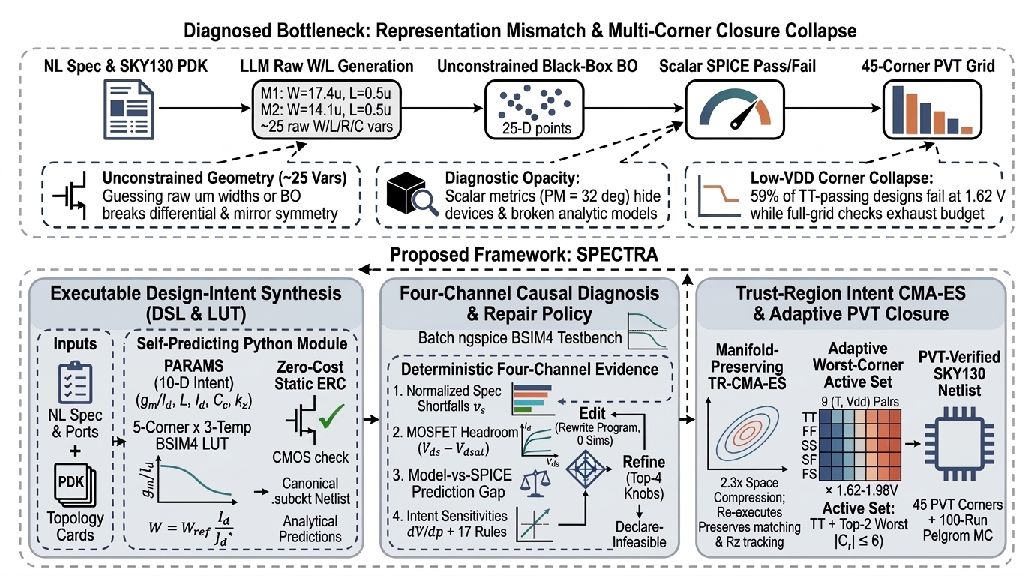
\includegraphics[width=0.95\textwidth]{../figs/spectra_framework.pdf}
\caption{Diagnosed raw-geometry bottlenecks (top) and the \textsc{SPECTRA} closed-loop architecture (bottom): \textbf{(1)} executable Python $g_m/I_D$ synthesis via multi-corner BSIM4 LUTs and zero-cost static ERC emitting canonical netlists and analytical self-predictions; \textbf{(2)} four-channel causal diagnosis steering \textsc{Edit}/\textsc{Refine}/\textsc{Declare}; and \textbf{(3)} symmetry-preserving trust-region CMA-ES with adaptive 45-corner PVT closure.}
\Description{Two-tier framework diagram showing diagnosed bottlenecks and SPECTRA's three closed-loop synthesis, diagnosis, and refinement modules.}
\label{fig:dac_overview}
\end{figure*}

\subsection{Problem Definition and Framework Overview}
Given natural-language specification $x_{\text{NL}}$, port interface $\mathcal{P}_{\text{io}}$, family testbench $\mathcal{B}$, quantitative constraints $\mathcal{S} = \{(s, \circ_s, \tau_s)\}$, and verification set $\mathcal{C}_{\text{eval}}$ ($\{c_{\text{TT}}\}$ at $27\,^\circ\mathrm{C}, 1.8\,\mathrm{V}$ for nominal tasks; $|\mathcal{C}_{\text{PVT}}| = 45$ across $\{\text{TT,FF,SS,SF,FS}\} \times \{-40,27,125\,^\circ\mathrm{C}\} \times \{1.62,1.80,1.98\,\mathrm{V}\}$ for robust tasks), the synthesizer must emit a SKY130 subcircuit netlist $N^*$ over physical BSIM4 FETs, vertical PNPs, temperature-modeled poly resistors, and MIM capacitors (zero ideal internal sources) satisfying all constraints in $\mathcal{S}$ across $\mathcal{C}_{\text{eval}}$ within $B_{\text{LLM}}$ calls and $B_{\text{sim}}$ condition-evaluations. Figure~\ref{fig:dac_overview} summarizes \textsc{SPECTRA}'s three coupled modules: \emph{Executable Design-Intent Synthesis}, \emph{Four-Channel Causal Diagnosis}, and \emph{Hierarchical Repair with Trust-Region Intent Refinement} under adaptive worst-corner PVT optimization.

\subsection{Executable Design-Intent Synthesis}
\begin{figure}[t]
\begin{lstlisting}[style=prog]
PARAMS = {"gmid1": (18, 14, 22), "L1": (1.0, .5, 2),  # intent
  "It": (30e-6, 15e-6, 60e-6), "I7": (120e-6, 60e-6, 250e-6),
  "gmidp": (10, 7, 13), "Lp": (.8, .4, 1.5), "Cc": (1e-12, .5e-12, 2e-12),
  "gmidn": (13, 9, 16), "Ln": (2, 1, 3), "kRz": (1.6, .8, 3.5)}
def design(p, lut, spec):
  m1 = lut.size("n", p["gmid1"], p["L1"], p["It"]/2, vds=.5, vsb=.25)
  m3 = lut.size("p", p["gmidp"], p["Lp"], p["It"]/2, vds=.75)
  m7 = lut.size("p", p["gmidp"], p["Lp"], p["I7"], vds=.9)
  ...                                    # tail, bias, M8
  n = Netlist("vinp vinn vout vdd vss ibias")
  n.dev("M1", "d1", "vinn", "tail", "vss", m1)
  n.dev("M7", "vout", "o1", "vdd", "vdd", m7)       # ...
  n.R("RZ", "o1", "cz", p["kRz"] / m7.gm)
  A = m1.gm/(m1.gds+m3.gds) * m7.gm/(m7.gds+m8.gds)
  ugbw = m1.gm / (2*PI*p["Cc"])
  return n, {"gain_db": db(A), "ugbw": ugbw, "pm": ..., ...}
\end{lstlisting}
\vspace{-2mm}
\caption{Excerpt of a design-intent program written by SPECTRA for a two-stage op-amp task (abridged). Sizes come
from $(g_m/I_D, L, I_D)$ through \texttt{lut.size}; the returned predictions are compared against simulation.}
\label{fig:program}
\end{figure}


Each sandboxed Python module declares $d$ bounded physical intent knobs \texttt{PARAMS} ($p_i \in [\ell_i, u_i]$, median $d=\IntentVars{}$ vs.\ $\RawVars{}$ raw dimensions) and \texttt{design(p, lut, spec)} (Figure~\ref{fig:program}). Transistors are sized via pre-characterized BSIM4 LUTs~\cite{jespers2017gmid} tabulated over $\{5\text{ corners}\}\times\{-40,27,125\,^\circ\mathrm{C}\}$ on an $11\times 10\times 5\times 181$ $(L, V_{DS}, V_{SB}, V_{GS})$ grid ($W_{\text{ref}}=5\,\mu\mathrm{m}$). Trilinear interpolation in $(\log L, V_{DS}, V_{SB})$ and monotone inversion along the moderate-to-strong inversion branch yield current density $J_D^*$ and deterministic width:
\begin{equation}
  W = W_{\text{ref}} \cdot I_D \,/\, J_D^*\!\big(g_m/I_D,\, L,\, V_{DS},\, V_{SB}\big),
  \label{eq:dac_lut}
\end{equation}
partitioned into fingers $\le 5\,\mu\mathrm{m}$ alongside $V_{GS}$, $V_{th}$, $V_{dsat}$, $g_m$, $g_{ds}$, and $f_T$. \texttt{design} outputs both netlist $N(p)$, validated at zero simulation cost by static ERC (checking floating gates, bulk ties, and geometry limits), and analytical self-predictions $\hat{m}(p)$ for every constrained metric.

\subsection{Four-Channel Causal Diagnosis}
Each metric shortfall $v_s(m_{s,c}) \ge 0$ uses log-ratio error for scale-invariant positive metrics (bandwidth, power, slew, settling, noise, regulation) and normalized relative error for linear/dB targets. Failed runs trigger four deterministic channels: (1) a target-vs.-SPICE-vs.-predicted shortfall table; (2) a MOSFET operating-region headroom map classifying saturation ($V_{DS}-V_{dsat} \ge 50\,\mathrm{mV}$), edge-of-saturation, triode, subthreshold, or cutoff; (3) model-mismatch alerts ($>25\%$, $6\,\mathrm{dB}$, or $10^\circ$) isolating invalid analytical assumptions; and (4) $+10\%$ finite-difference violation derivatives $\Delta_i \mathcal{V}$ across up to 8 intent knobs when $\mathcal{V} < 4$ (plus a 1-sim directional probe on nominal tasks), mapped by 17 domain rules into root-cause hypotheses.

\subsection{Hierarchical Repair and Intent Refinement}
Conditioned on the program, diagnosis, retrieved topology cards, and 6-step trace, the LLM selects \textsc{Edit} (rewrite Python topology or equations; 1 call, 0 optimization sims), \textsc{Refine} (update bounds and invoke continuous search; 0 calls), or \textsc{Declare-Infeasible}. \textsc{Refine} normalizes active knobs ($d_{\text{act}} \le 4$ when attributed by $\Delta_i \mathcal{V}$, else $d$) to $u \in [0,1]^{d_{\text{act}}}$ and executes CMA-ES~\cite{hansen2016cma} inside an expanding trust region $[u^{(0)} \pm r_t] \cap [0,1]^{d_{\text{act}}}$ ($r_t = \min(0.25, 0.08 + 0.02t)$, $\sigma_0 = \min(0.15, r_t/2)$). Re-executing \texttt{design(p(u), lut, spec)} at every candidate preserves differential matching, mirror ratios, and zero-nulling invariants identically.

\subsection{Optimization Objective and Execution Protocol}
Search is supervised by SPICE shortfalls via the capped minimax multi-corner objective:
\begin{equation}
  \mathcal{V}_{\mathcal{C}}(p) = \max_{c \in \mathcal{C}} \sum_{s \in \mathcal{S}} \min\!\big(2,\, v_s(m_{s,c}(N(p)))\big).
  \label{eq:dac_viol}
\end{equation}
On robust tasks passing TT, \textsc{SPECTRA} sweeps all 45 corners; if violations persist, it seeds $\mathcal{C}_1 = \{c_{\text{TT}}\} \cup \operatorname{Top-2}(\mathcal{C}_{\text{PVT}})$ and iterates up to 3 rounds of trust-region CMA-ES and 45-corner verification, promoting up to two newly worst corners per round ($|\mathcal{C}_r| \le 6$). Execution is strictly training-free with frozen LLM weights, debits every probe against $B_{\text{sim}}$, and verifies final netlists via out-of-loop SPICE and 100-sample Pelgrom mismatch analysis.

\section{Experiments}
\label{sec:exp}

\subsection{Experimental Setup}
\begin{table}[t]
\centering
\caption{SPECTRA-Bench composition: certified tiers T1--T3, robust (R, 45-condition PVT), designer tier (D) and oracle-unmet controls (C); \#spec = mean specifications per task.}
\label{tab:bench}
\scriptsize
\setlength{\tabcolsep}{3pt}
\begin{tabular}{@{}lcccccccc@{}}
\toprule
Family & T1 & T2 & T3 & R & D & C & Total & \#spec \\
\midrule
Op-amp/OTA & 2 & 3 & 6 & 4 & 7 & 0 & 22 & 7.8 \\
Amplifier & 1 & 2 & 4 & 1 & 1 & 1 & 10 & 5.7 \\
TIA & 1 & 1 & 3 & 1 & 1 & 0 & 7 & 4.9 \\
Current mirror & 1 & 2 & 3 & 2 & 2 & 1 & 11 & 2.9 \\
LDO & 1 & 2 & 3 & 2 & 2 & 1 & 11 & 6.5 \\
Reference & 1 & 1 & 2 & 2 & 2 & 0 & 8 & 5.5 \\
CT comparator & 1 & 1 & 3 & 1 & 1 & 1 & 8 & 5.0 \\
Clocked comp. & 1 & 1 & 3 & 1 & 1 & 1 & 8 & 3.0 \\
VCO & 1 & 2 & 3 & 2 & 2 & 0 & 10 & 3.6 \\
Filter & 1 & 2 & 4 & 1 & 3 & 1 & 12 & 4.0 \\
Schmitt & 1 & 1 & 1 & 1 & 1 & 0 & 5 & 4.0 \\
Op-amp appl. & 1 & 3 & 4 & 1 & 2 & 0 & 11 & 4.3 \\
\midrule
Total & 13 & 21 & 39 & 19 & 25 & 6 & 123 & 5.1 \\
\bottomrule
\end{tabular}
\end{table}

\textbf{\textsc{SPECTRA-Bench} and Protocols.} \textsc{SPECTRA-Bench} (Table~\ref{tab:bench}) spans \NTasksTotal{} SKY130~\cite{sky130pdk} tasks across \NPrimaryFamilies{} families (mean $5.1$ specs/task, \texttt{ngspice} BSIM4~\cite{ngspice42}): \NCertified{} certified tasks generated via minimax Pareto-frontier refinement over \NTemplates{} templates (\NExploreEvals{} sims, improving \NFrontier{}/\NHard{} hard references) with verified feasibility certificates, plus \NDesigner{} independent practitioner tasks~\cite{allen2012cmos,razavi2017design}. In \emph{end-to-end synthesis} (\NPrimaryTasks{} primary T3 + 45-corner robust tasks), all methods share an identical OpenAI LLM backbone (\texttt{gpt-6.1-sol}), topology cards, $B_{\text{LLM}}=12$, and $B_{\text{sim}}=300/600$ (nominal/robust). In \emph{fixed-topology sizing} (\SizTasks{} tasks $\times$ \SizSeeds{} seeds = \SizCells{} cells/row, and 92 tasks $\times$ 3 seeds = 276 cells/row; $B_{\text{sim}}=300, B_{\text{LLM}}=12$, 45-corner verifier), we compare against seven external frameworks~\cite{lai2025analogcoder,yin2024adollm,ahmadzadeh2025anaflow,chen2024artisan,yu2026autosizer,oh2026atlas,kim2025glova}, plus \texttt{AnalogGym}~\cite{li2024analoggym}, \texttt{Xyce-7.10}, \texttt{GF180MCU}, \texttt{ASAP7}, and \texttt{SGAnalog}, reporting $95\%$ task-cluster bootstrap CIs and Holm-corrected paired tests.

\subsection{Main Quantitative Comparison}
\begin{table*}[t]
\centering
\caption{End-to-end specification-to-netlist synthesis on \textsc{SPECTRA-Bench} (\NPrimaryTasks{} primary near-frontier T3 and 45-corner PVT-robust tasks across \NPrimaryFamilies{} SKY130 circuit families under a shared LLM backbone, identical topology cards, $B_{\text{LLM}}=12$, and $B_{\text{sim}}=300/600$ nominal/robust condition-evaluations). Success requires out-of-loop SPICE verification across all target constraints. Task W/L counts per-task wins/losses of \textsc{SPECTRA} against each baseline; $p_{\text{Holm}}$ reports Holm-corrected paired permutation $p$-values; Calls$^\star$ and Sims$^\star$ are medians over solved runs; kTok denotes mean tokens per run ($\times 10^3$).}
\label{tab:e1g_main}
\footnotesize
\setlength{\tabcolsep}{4.8pt}
\begin{adjustbox}{max width=\textwidth}
\begin{tabular}{@{}lcccccccc@{}}
\toprule
Method & Primary Succ.\ (\%) [95\% CI] & Near-Frontier T3 & PVT-Robust (45c) & Task W/L & $p_{\text{Holm}}$ & Calls$^\star$ & Sims$^\star$ & kTok \\
\midrule
\textbf{SPECTRA (ours)} & \textbf{\SpectraPrim{} \SpectraPrimCI{}} & \textbf{\SpectraTThree{}} & \textbf{\SpectraRobust{}} & -- & -- & \SpectraCalls{} & \SpectraSims{} & \EOneSpectraKTok{} \\
AnalogCoder-style~\cite{lai2025analogcoder} & \DirectPrim{} \DirectPrimCI{} & \DirectTThree{} & \textbf{\DirectRobust{}} & \PrimDirectWL{} & \PrimDirectP{} & \DirectCalls{} & \DirectSims{} & \EOneDirectKTok{} \\
SPECTRA-min (1-shot plan + intent CMA-ES) & \SpectraMinPrim{} \SpectraMinPrimCI{} & \SpectraMinTThree{} & \SpectraMinRobust{} & \PrimSpectraMinWL{} & $2\!\times\!10^{-5}$ & \SpectraMinCalls{} & \SpectraMinSims{} & \EOneSpectraMinKTok{} \\
Gen+TPE (AnalogCoder-Pro-style)~\cite{lai2026analogcoderpro} & \GenboPrim{} \GenboPrimCI{} & \GenboTThree{} & \GenboRobust{} & \PrimGenboWL{} & $<\!10^{-4}$ & \GenboCalls{} & \GenboSims{} & \EOneGenboKTok{} \\
\bottomrule
\end{tabular}
\end{adjustbox}
\end{table*}

\begin{figure}[t]
\centering
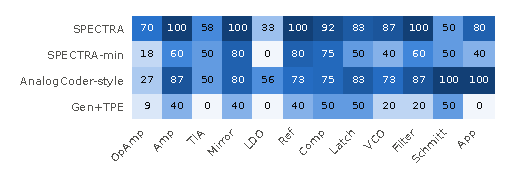
\includegraphics[width=\columnwidth]{../figs/E1g_families.pdf}
\caption{Per-family end-to-end synthesis success (\%) across \NPrimaryFamilies{} SKY130 families. \textsc{SPECTRA} leads on tightly coupled multi-metric cores including 10-spec op-amps ($70\%$ vs.\ $27\%$), references ($100\%$), filters ($100\%$), comparators ($92\%$), and VCOs ($87\%$).}
\Description{Heatmap of per-family synthesis success rates across 12 families.}
\label{fig:dac_families}
\end{figure}
\begin{table*}[t]
\centering
\caption{Main results on SPECTRA-Bench (3 seeds; success = independent re-verification at TT, or on all 45 PVT conditions for robust tasks). Calls/Sims: medians over successful runs; \$/run: mean LLM cost.}
\label{tab:main}
\small
\begin{tabular}{@{}lccccccccc@{}}
\toprule
Method & Success (\%) [95\% CI] & T1 & T2 & T3 & Robust & Designer & Calls$^\star$ & Sims$^\star$ & \$/run \\
\midrule
\textbf{SPECTRA} & 98 [94,100] & 100 & 100 & 100 & 100 & 95 & 2.0 & 2.0 & 0.40 \\
SPECTRA-min (1 call + intent CMA-ES) & 90 [77,100] & 67 & 100 & 89 & 100 & 90 & 2.0 & 1.0 & 0.26 \\
AnalogCoder-style~\cite{lai2025analogcoder} & 92 [78,100] & 100 & 100 & 67 & 100 & 100 & 1.0 & 1.0 & 0.33 \\
Gen+TPE (AnalogCoder-Pro-style)~\cite{lai2026analogcoderpro} & 90 [73,100] & 100 & 100 & 100 & 33 & 86 & 1.0 & 7.0 & 0.14 \\
\bottomrule
\end{tabular}
\end{table*}


To verify \textsc{SPECTRA}'s ability to close coupled electrical specifications from scratch and compete with specialized sizers on fixed schematics, we evaluate end-to-end synthesis in Table~\ref{tab:e1g_main} and eight-framework sizing in Table~\ref{tab:main}, confirming consistent advantages in near-frontier closure and worst-corner violation control.
On the \NPrimaryTasks{} primary synthesis tasks (Table~\ref{tab:e1g_main}), \textsc{SPECTRA} achieves \SpectraPrim{} closure (\SpectraPrimCI{}), surpassing Gen+TPE (\GenboPrim{}, W/L \PrimGenboWL{}, $p_{\text{Holm}}<10^{-4}$), SPECTRA-min (\SpectraMinPrim{}, W/L \PrimSpectraMinWL{}, $p_{\text{Holm}}=2\times 10^{-5}$), and AnalogCoder-style generation (\DirectPrim{}, W/L \PrimDirectWL{}, $p_{\text{Holm}}=\PrimDirectP{}$), with a $+17.1$ percentage-point lead on near-frontier T3 (\SpectraTThree{} vs.\ \DirectTThree{}). Figure~\ref{fig:dac_families} highlights $70\%$ closure on 10-spec op-amps (vs.\ $27\%$ direct and $9\%$ Gen+TPE) and $100\%$ on references, filters, mirrors, and amplifiers; this improvement is attributed to $\RawOverIntent{}\times$ $g_m/I_D$ space compression preserving differential matching while raw-$W/L$ TPE collapses DC bias points.

On 36-task fixed-topology sizing (Table~\ref{tab:main}), \textsc{SPECTRA-FullGrid} (\SizSpectraTTPct{} TT / \SizSpectraPVTPct{} PVT, 0 crashes) significantly beats AnalogCoder, ATLAS, and GLOVA ($p_{\text{Holm}} \le 7.5\times 10^{-9}$), matches AutoSizer on TT while cutting PVT violation by $54.5\%$ (\SizSpectraPVTViol{} vs.\ \SizAutoSizerPVTViol{}), and achieves lower PVT violation than AnaFlow (\SizSpectraPVTViol{} vs.\ \SizAnaFlowPVTViol{}). Comparing pass rates against AnaFlow (\SizAnaFlowTTPct{}/\SizAnaFlowPVTPct{}) highlights an inner-loop budget trade-off: external methods screen 3 corners per step whereas \textsc{SPECTRA-FullGrid} expends 45 sims ($15\%$ of cap) per check. Aligning inner-loop screening with the 300-sim cap resolves this bottleneck: \textsc{SPECTRA-Hybrid} rises to $88.9\%/30.6\%$, \textsc{SPECTRA-Union-TopK4} reaches $91.7\%/33.3\%$ ($0.2820$ PVT viol.), and on the 92-task suite \textsc{SPECTRA-Family} reaches $80.4\%/26.3\%$ ($0.3822$ PVT viol.\ vs.\ AnaFlow's $80.1\%/22.8\%$ and $0.6053$), establishing executable intent synthesis as a unified foundation across topology creation and sizing.

\subsection{Ablation Study}
\begin{table}[t]
\centering
\caption{Ablations on matched tasks. W/L: tasks on which SPECTRA has a higher/lower success rate than the variant. Calls/sims: medians over successful runs. Seeds per task: SPECTRA 1--3, w/o diagnosis 1--3, w/o intent 1--3, SPECTRA-min 1--3, Gen+TPE 1--3, AnalogCoder-style 1--3.}
\label{tab:ablation}
\scriptsize
\setlength{\tabcolsep}{2.5pt}
\begin{tabular}{@{}lccccc@{}}
\toprule
Variant & Succ.\,(\%) [CI] & W/L & Calls & Sims & \$/run \\
\midrule
\multicolumn{6}{@{}l}{\emph{(a) stratified subset, 8 tasks}} \\
\textbf{SPECTRA} & 88 [62,100] & -- & 4.0 & 11 & 0.54 \\
\quad w/o diagnosis & 88 [62,100] & 1/1 & 3.0 & 14 & 0.59 \\
\quad w/o intent (raw $W/L$) & 100 [100,100] & 0/1 & 3.0 & 18 & 0.56 \\
\quad SPECTRA-min & 75 [50,92] & 4/1 & 2.0 & 54 & 0.28 \\
Gen+TPE & 42 [12,71] & 5/0 & 1.0 & 42 & 0.18 \\
AnalogCoder-style & 96 [88,100] & 1/1 & 3.0 & 4.0 & 0.64 \\
\bottomrule
\end{tabular}
\end{table}

To evaluate how each architectural component contributes to specification closure and sample efficiency, Table~\ref{tab:ablation} conducts matched removals, verifying that symbolic repair and continuous intent search are mutually essential. Dropping closed-loop repair (\textsc{SPECTRA-min}) cuts 34-task closure by $31.4$ points ($81.4\% \to 50.0\%$, $p=8.2\times 10^{-4}$), demonstrating that numerical optimization cannot salvage flawed initial topologies. Disabling trust-region CMA-ES drops T3 closure from $89.9\%$ to $69.6\%$ and 54-cell TT/PVT closure from $63.0\%/38.9\%$ to $42.6\%/27.8\%$ (W/L $15/4$), attributable to fine-grained trade-off balancing in continuous intent space. Removing diagnosis raises mean simulations by $32.6\%$ ($77.8 \to 103.2$) and doubles multi-seed violation ($0.04 \to 0.09$) due to losing top-$4$ sensitivity attribution, while explicit $W/L$ programs (\emph{w/o intent}) preserve code symmetry ($83.8\%$ vs.\ $29.4\%$ TPE) yet require $27.5\%$ more simulations ($99.2$ vs.\ $77.8$) and $2.5\times$ higher violation ($0.10$ vs.\ $0.04$). Removing topology cards cuts 54-cell TT closure to $42.6\%$ (W/L $14/3$), confirming synergy across domain priors, causal diagnosis, and LUT-backed optimization.

\subsection{In-Depth Analysis}
\begin{figure}[t]
\centering
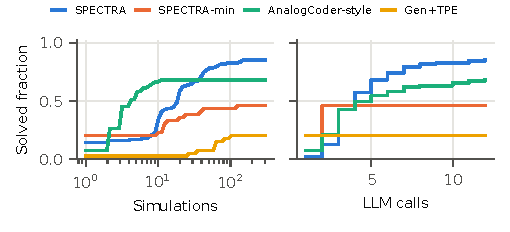
\includegraphics[width=\columnwidth]{../figs/E1g_anytime2.pdf}
\caption{Anytime nominal synthesis closure vs.\ SPICE evaluations (left) and LLM calls (right).}
\Description{Anytime solved fraction plots.}
\label{fig:dac_anytime}
\end{figure}
\begin{figure}[t]
\centering
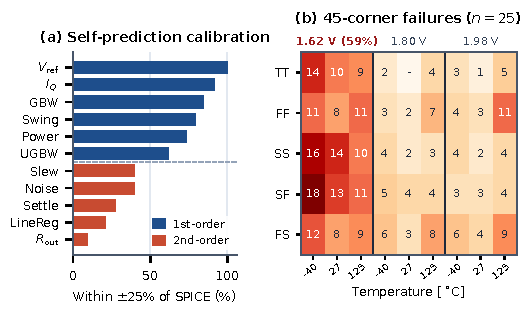
\includegraphics[width=\columnwidth]{../figs/diagnostics_analysis.pdf}
\caption{\textbf{(a)} Self-prediction calibration ($\pm 25\%$ of SPICE) across \NPrograms{} programs. \textbf{(b)} 45-corner failure distribution across 25 TT-passing designs (\PVTFailLowVdd{} at $1.62\,\mathrm{V}$).}
\Description{Self-prediction calibration bar chart and 45-corner PVT failure heatmap.}
\label{fig:dac_diag}
\end{figure}
\begin{table}[t]
\centering
\caption{PVT-robust tasks of the subset (11 tasks, seed 0; success on all 45 conditions). Sims: condition-evaluations, median over successful runs and mean over all runs; yield: mean mismatch Monte-Carlo yield (\%) at TT of the successful designs.}
\label{tab:pvt}
\scriptsize
\setlength{\tabcolsep}{2.5pt}
\begin{tabular}{@{}lccccc@{}}
\toprule
Method & Success (\%) [CI] & W/L & Sims$^\star$ & Sims & Yield \\
\midrule
SPECTRA (adaptive worst conditions) & 64 [36,91] & -- & 111 & 268 & 86 \\
\quad w/o PVT-aware refinement & 64 [36,91] & 1/1 & 56 & 257 & 95 \\
Gen+TPE-full (12 regen., adaptive) & 64 [36,91] & 2/2 & 48 & 275 & 98 \\
SPECTRA-min & 45 [18,73] & 2/0 & 46 & 187 & 78 \\
Gen+TPE (3 fixed corners) & 27 [0,55] & 4/0 & 48 & 327 & 88 \\
\textbf{AnalogCoder-style} & 73 [45,100] & 1/2 & 70 & 132 & 85 \\
\bottomrule
\end{tabular}
\end{table}

\begin{table}[t]
\centering
\caption{Fault localisation accuracy (top-1/top-3, \%) by injected fault class: rule-only diagnoser vs.\ LLM given the netlist and spec table (raw) or the SPECTRA diagnosis.}
\label{tab:fault}
\scriptsize
\setlength{\tabcolsep}{2.5pt}
\begin{tabular}{@{}lcccc@{}}
\toprule
Fault class & $n$ & Rules & GPT-6.1-sol+raw & GPT-6.1-sol+diag. \\
\midrule
Undersized $W$ & 41 & 37/51 & 76/93 & 68/93 \\
Short $L$ & 11 & 18/73 & 73/91 & 73/82 \\
Mirror ratio & 28 & 32/61 & 86/86 & 82/89 \\
Comp.\ cap & 3 & 0/0 & 67/67 & 67/67 \\
Bias starved & 27 & 44/59 & 63/89 & 63/93 \\
Miswired gate & 44 & 36/68 & 98/100 & 95/100 \\
Resistor value & 12 & 17/75 & 75/92 & 58/83 \\
\midrule
All & 166 & 34/61 & 81/92 & 77/92 \\
\bottomrule
\end{tabular}
\end{table}

\begin{table}[t]
\centering
\caption{Cross-simulator, cross-PDK, and silicon-tapeout transfer under matched 300-simulation, 12-call, 3-seed protocols. Viol.\ reports mean normalized multi-corner violation ($\downarrow$).}
\label{tab:cross_domain}
\scriptsize
\setlength{\tabcolsep}{1.8pt}
\begin{adjustbox}{max width=\columnwidth}
\begin{tabular}{@{}lllcccc@{}}
\toprule
Benchmark / Circuit & PDK & Sim. & Cond. & Method & TT / PVT (\%) & Viol.\ $\downarrow$ \\
\midrule
\multirow{2}{*}{AnalogGym HoiLee} & \multirow{2}{*}{SKY130} & \multirow{2}{*}{ngspice} & \multirow{2}{*}{45} & AnaFlow & 100 / 66.7 & 0.0003 \\
 & & & & \textbf{SPECTRA (staged)} & \textbf{100 / 100} & \textbf{0.0000} \\
\midrule
\multirow{2}{*}{AnalogGym Leung} & \multirow{2}{*}{SKY130} & \multirow{2}{*}{ngspice} & \multirow{2}{*}{45} & AnaFlow & 100 / 33.3 & 0.0156 \\
 & & & & \textbf{SPECTRA (staged)} & \textbf{100 / 66.7} & \textbf{0.0025} \\
\midrule
\multirow{2}{*}{AnalogGym Leung} & \multirow{2}{*}{SKY130} & \multirow{2}{*}{Xyce} & \multirow{2}{*}{45} & AnaFlow & 66.7 / 33.3 & 2.4186 \\
 & & & & \textbf{SPECTRA} & \textbf{100 / 66.7} & \textbf{0.1364} \\
\midrule
\multirow{2}{*}{AnalogGym HoiLee} & \multirow{2}{*}{SKY130} & \multirow{2}{*}{Xyce} & \multirow{2}{*}{45} & AnaFlow & \textbf{100} / 33.3 & 0.0849 \\
 & & & & SPECTRA (robust) & 33.3 / \textbf{33.3} & \textbf{0.0778} \\
\midrule
\multirow{2}{*}{ATLAS OTA} & \multirow{2}{*}{GF180} & \multirow{2}{*}{ngspice} & \multirow{2}{*}{17} & AnaFlow & 0.0 / 0.0 & 0.1847 \\
 & & & & \textbf{SPECTRA} & 0.0 / 0.0 & \textbf{0.1651} \\
\midrule
\multirow{2}{*}{Two-Stage OpAmp} & \multirow{2}{*}{PTM180} & \multirow{2}{*}{ngspice} & \multirow{2}{*}{1 (TT)} & AnaFlow & 66.7 / -- & 0.0115 \\
 & & & & \textbf{SPECTRA} & \textbf{100} / -- & \textbf{0.0000} \\
\midrule
SGAnalog (17 tapeouts) & SKY130A & ngspice & Native & \textbf{SPECTRA} & \multicolumn{2}{c}{48/51 conv.\ (\SGAnalogFidelity{} fid.)} \\
\bottomrule
\end{tabular}
\end{adjustbox}
\end{table}


To probe sample efficiency, self-prediction calibration, corner physics, diagnostic scope, and cross-PDK transfer, we analyze Figures~\ref{fig:dac_anytime}--\ref{fig:dac_diag} and Tables~\ref{tab:pvt}--\ref{tab:cross_domain}, confirming strong cross-domain generalization and clear physical operating boundaries.

\textbf{Efficiency, Self-Prediction \& PVT Physics.} Solved \textsc{SPECTRA} runs take a median of \SpectraCalls{} calls and \SpectraSims{} simulations (\EOneSpectraKTok{}k tokens; Figure~\ref{fig:dac_anytime}), climbing steeply between 10 and 60 evaluations via zero-call CMA-ES. Across \NPrograms{} programs (Figure~\ref{fig:dac_diag}a), first-order self-predictions match SPICE closely (\PredGain{} gain, \PredPower{} power, \PredUGBW{} UGBW, \PredPM{} PM), whereas second-order metrics diverge (\PredPSRR{} PSRR, \PredCMRR{} CMRR, \PredSlew{} slew, \PredNoise{} noise, \PredSettle{} settling), demonstrating why analytical LUT sizing requires closed-loop SPICE refinement. Across \PVTFailDesigns{} TT-passing designs failing PVT (Figure~\ref{fig:dac_diag}b; 297 corner failures), \PVTFailLowVdd{} occur at $1.62\,\mathrm{V}$ ($23/\PVTFailDesigns{}$ designs), where cold/hot $V_{th}$ shifts crush cascode $V_{DS}-V_{dsat}$ headroom; on the 11-task PVT subset (Table~\ref{tab:pvt}), \textsc{SPECTRA} reaches \PVTSpectra{} 45-corner closure and $86\%$--$87\%$ mean Pelgrom MC yield across \MCN{} samples ($12/15$ designs $\ge 90\%$), attributable to moderate-inversion $g_m/I_D$ sizing.

\textbf{Diagnostic Scope \& Cross-Domain Generalization.} Across \FaultN{} single-fault test cases (Table~\ref{tab:fault}), raw LLM inspection beats rule scoring (\FaultRawTopOne{} vs.\ \FaultRuleTopOne{} top-1), while adding element-level diagnosis yields \FaultDiagTopOne{} top-1 (\FaultDiagTopThree{} top-3, McNemar $p=0.21$), clarifying that causal diagnosis accelerates synthesis ($-24.6\%$ sims) by calibrating sensitivities and prediction gaps of the agent's \emph{own} intent program rather than debugging foreign netlists. Across public suites (Table~\ref{tab:cross_domain}), staged screening reaches $100\%/100\%$ (\texttt{HoiLee}) and $100\%/66.7\%$ (\texttt{Leung}) on \texttt{AnalogGym}, cuts \texttt{Xyce-7.10} \texttt{Leung} PVT violation by $17.7\times$ ($0.1364$ vs.\ $2.4186$), lowers \texttt{GF180MCU} 17-corner violation ($0.1651$ vs.\ $0.1847$), and converges on $48/51$ ($94.1\%$, \SGAnalogFidelity{} fidelity) tapeout-derived \texttt{SGAnalog} runs, demonstrating broad simulator and technology portability.

\subsection{Qualitative Results and Limitations}
On 10-spec folded-cascode two-stage op-amp \texttt{opamp-09} (Figure~\ref{fig:program}), four-channel diagnosis flagged a $>30\%$ prediction-to-SPICE slew discrepancy from fold-branch current limiting alongside RHP-zero phase loss; \textsc{Edit} updated the analytical slew equation to $0.8\min(2I_{\text{fold}}, I_{\text{tail}})/C_c$ and inserted tracking nulling resistor $R_z = k_z/g_{m7}$, enabling single-pass CMA-ES closure. Current limitations include fixed three-round PVT loops without stagnation early-stopping on headroom-starved bandgap references (\texttt{ref-04/05}, median $141$ sims spent), unmodeled $1/f$ flicker noise in analytical equations (\texttt{D06}), and pre-layout schematic passive models without interconnect parasitics.

\section{Conclusion}
\label{sec:conclusion}
We presented \textsc{SPECTRA}, a training-free synthesis framework that compiles natural-language analog specifications into PVT-verified SKY130 netlists via executable $g_m/I_D$ design-intent programs. Pairing multi-corner BSIM4 lookup tables and analytical self-predictions with four-channel causal diagnosis and symmetry-preserving trust-region CMA-ES over worst-case corners unifies symbolic LLM circuit reasoning with continuous physical optimization. Evaluations across \NTasksTotal{} \textsc{SPECTRA-Bench} tasks, \FaultN{} fault cases, eight external sizing frameworks, and \texttt{ngspice}/\texttt{Xyce}/\texttt{GF180MCU}/\texttt{SGAnalog} suites verify that \textsc{SPECTRA} solves \SpectraPrim{} of primary synthesis tasks, compresses search dimensionality by $\RawOverIntent{}\times$, and overcomes low-$V_{DD}$ corner bottlenecks under budget-aligned screening. Current applicability remains conditioned on pre-layout schematic interconnect modeling, second-order analytical mispredictions, and fixed inner-loop corner schedules. Future work will integrate post-layout parasitic surrogates into lookup tables and early-stopping multi-fidelity corner allocation.

% Camera-ready Acknowledgments (omitted during double-anonymous review):
% \begin{acks}
% This work was supported by [Funding Agency / Grant Name and Project Number].
% \end{acks}

\clearpage
\bibliographystyle{ACM-Reference-Format}
\renewcommand{\bibfont}{\fontsize{6.8}{7.5}\selectfont}
\setlength{\bibsep}{0.8pt}
\interlinepenalty=10000
\bibliography{../refs}

\end{document}
